\chapter{Ingénierie des exigences}
\section{Approche Top-Down}
\label{sec:top-down}
\begin{figure}[h]
  \centering
  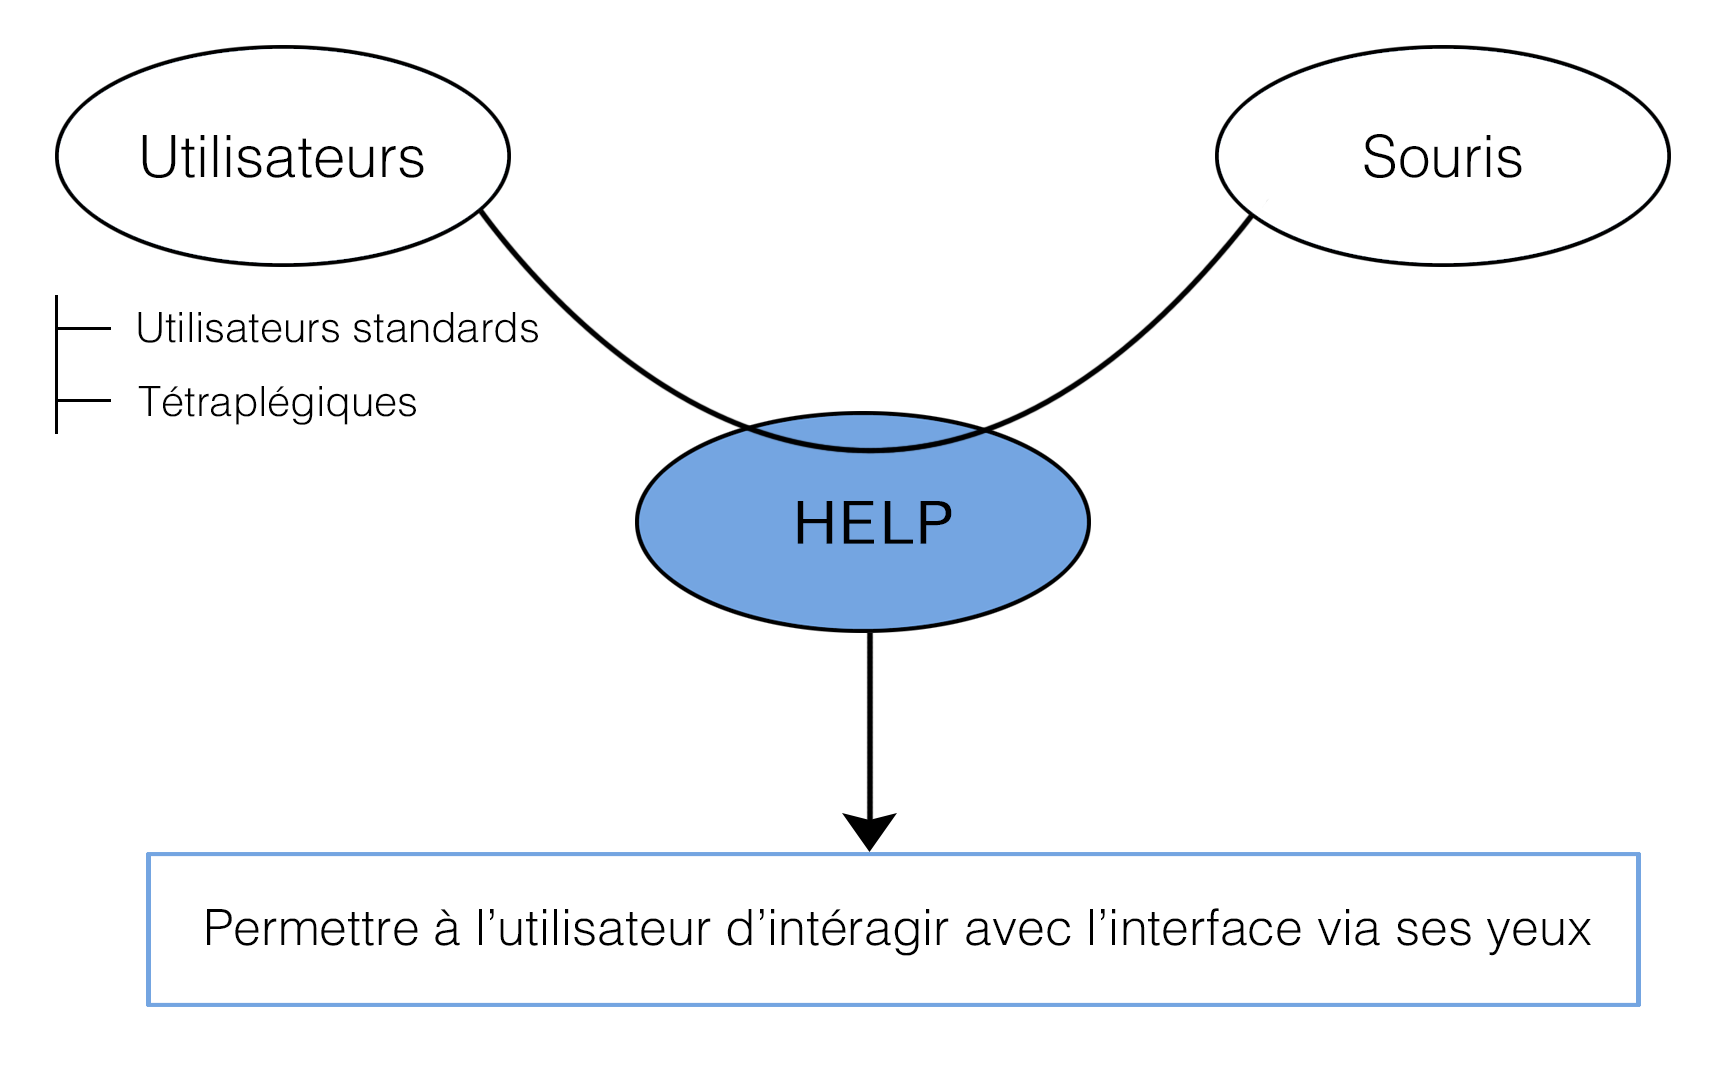
\includegraphics[scale=1]{BeteACornes}
  \caption{Bête à cornes}
  \label{fig:bac}
\end{figure}

\begin{figure}[H]
  \centering
  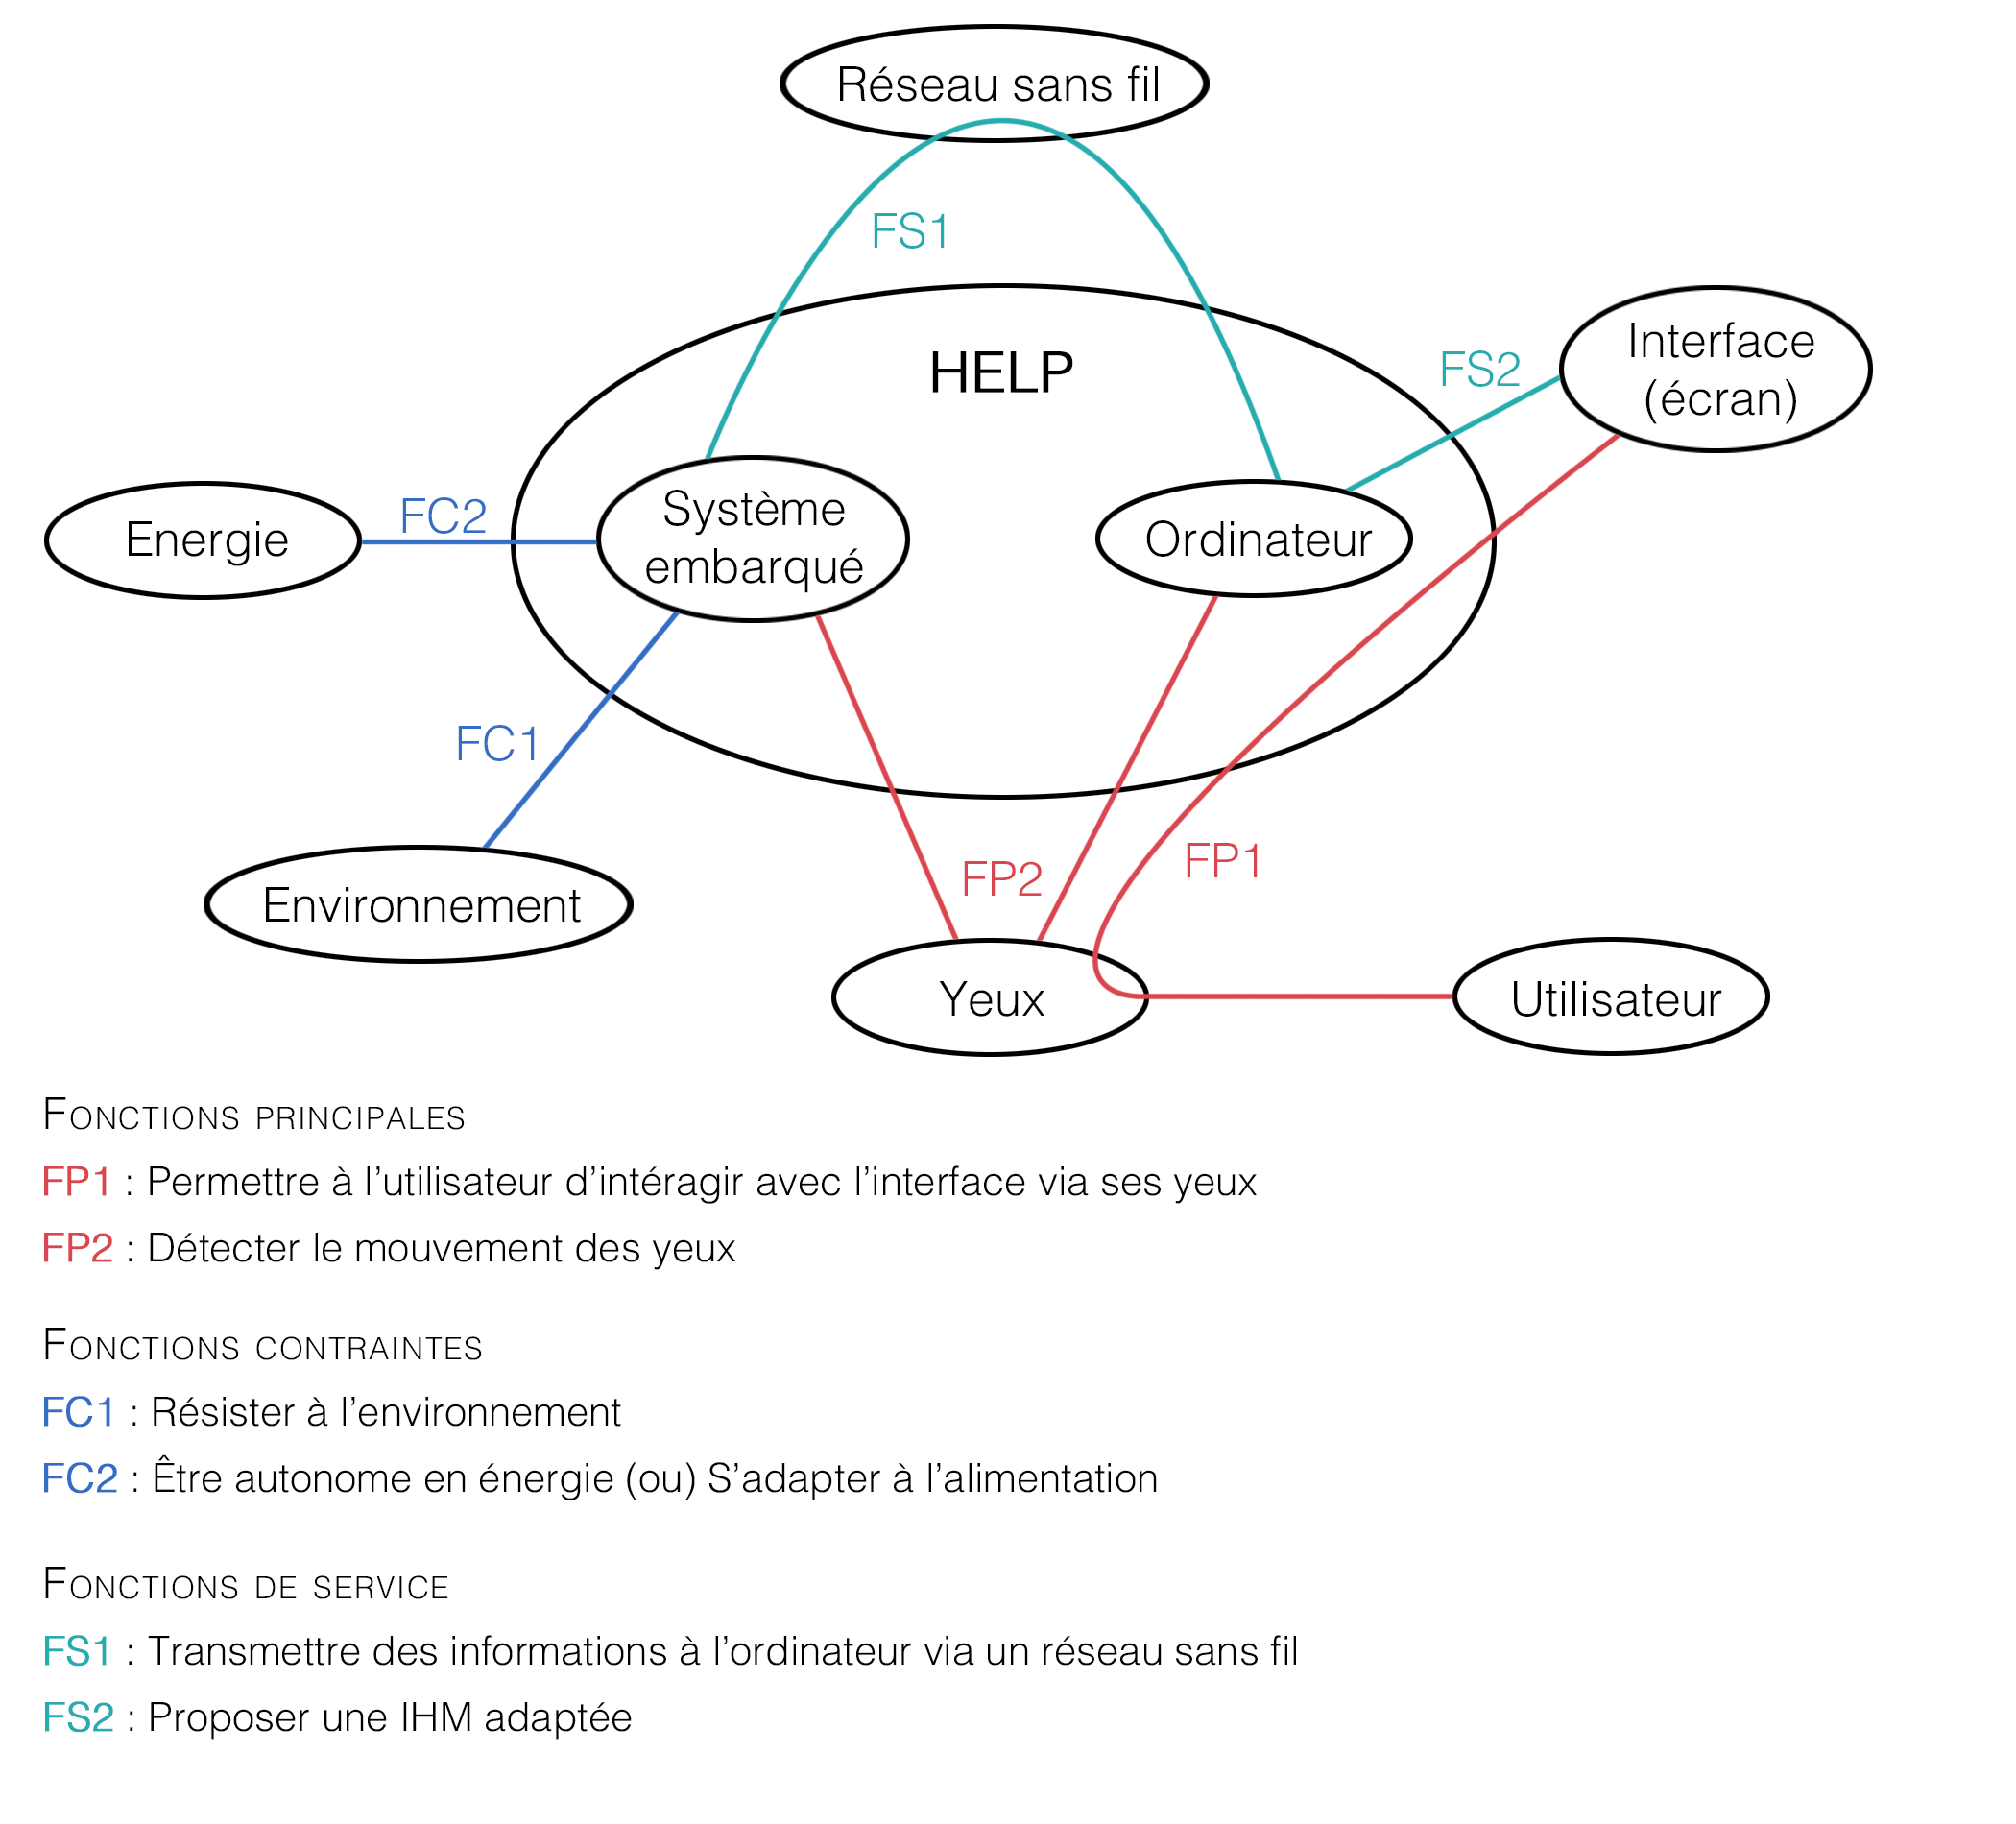
\includegraphics[scale=0.9]{Pieuvre}
  \caption{Diagramme pieuvre}
  \label{fig:pieuvre}
\end{figure}

\section{Approche Bottom-Up}

\begin{figure}[H]
  \centering
  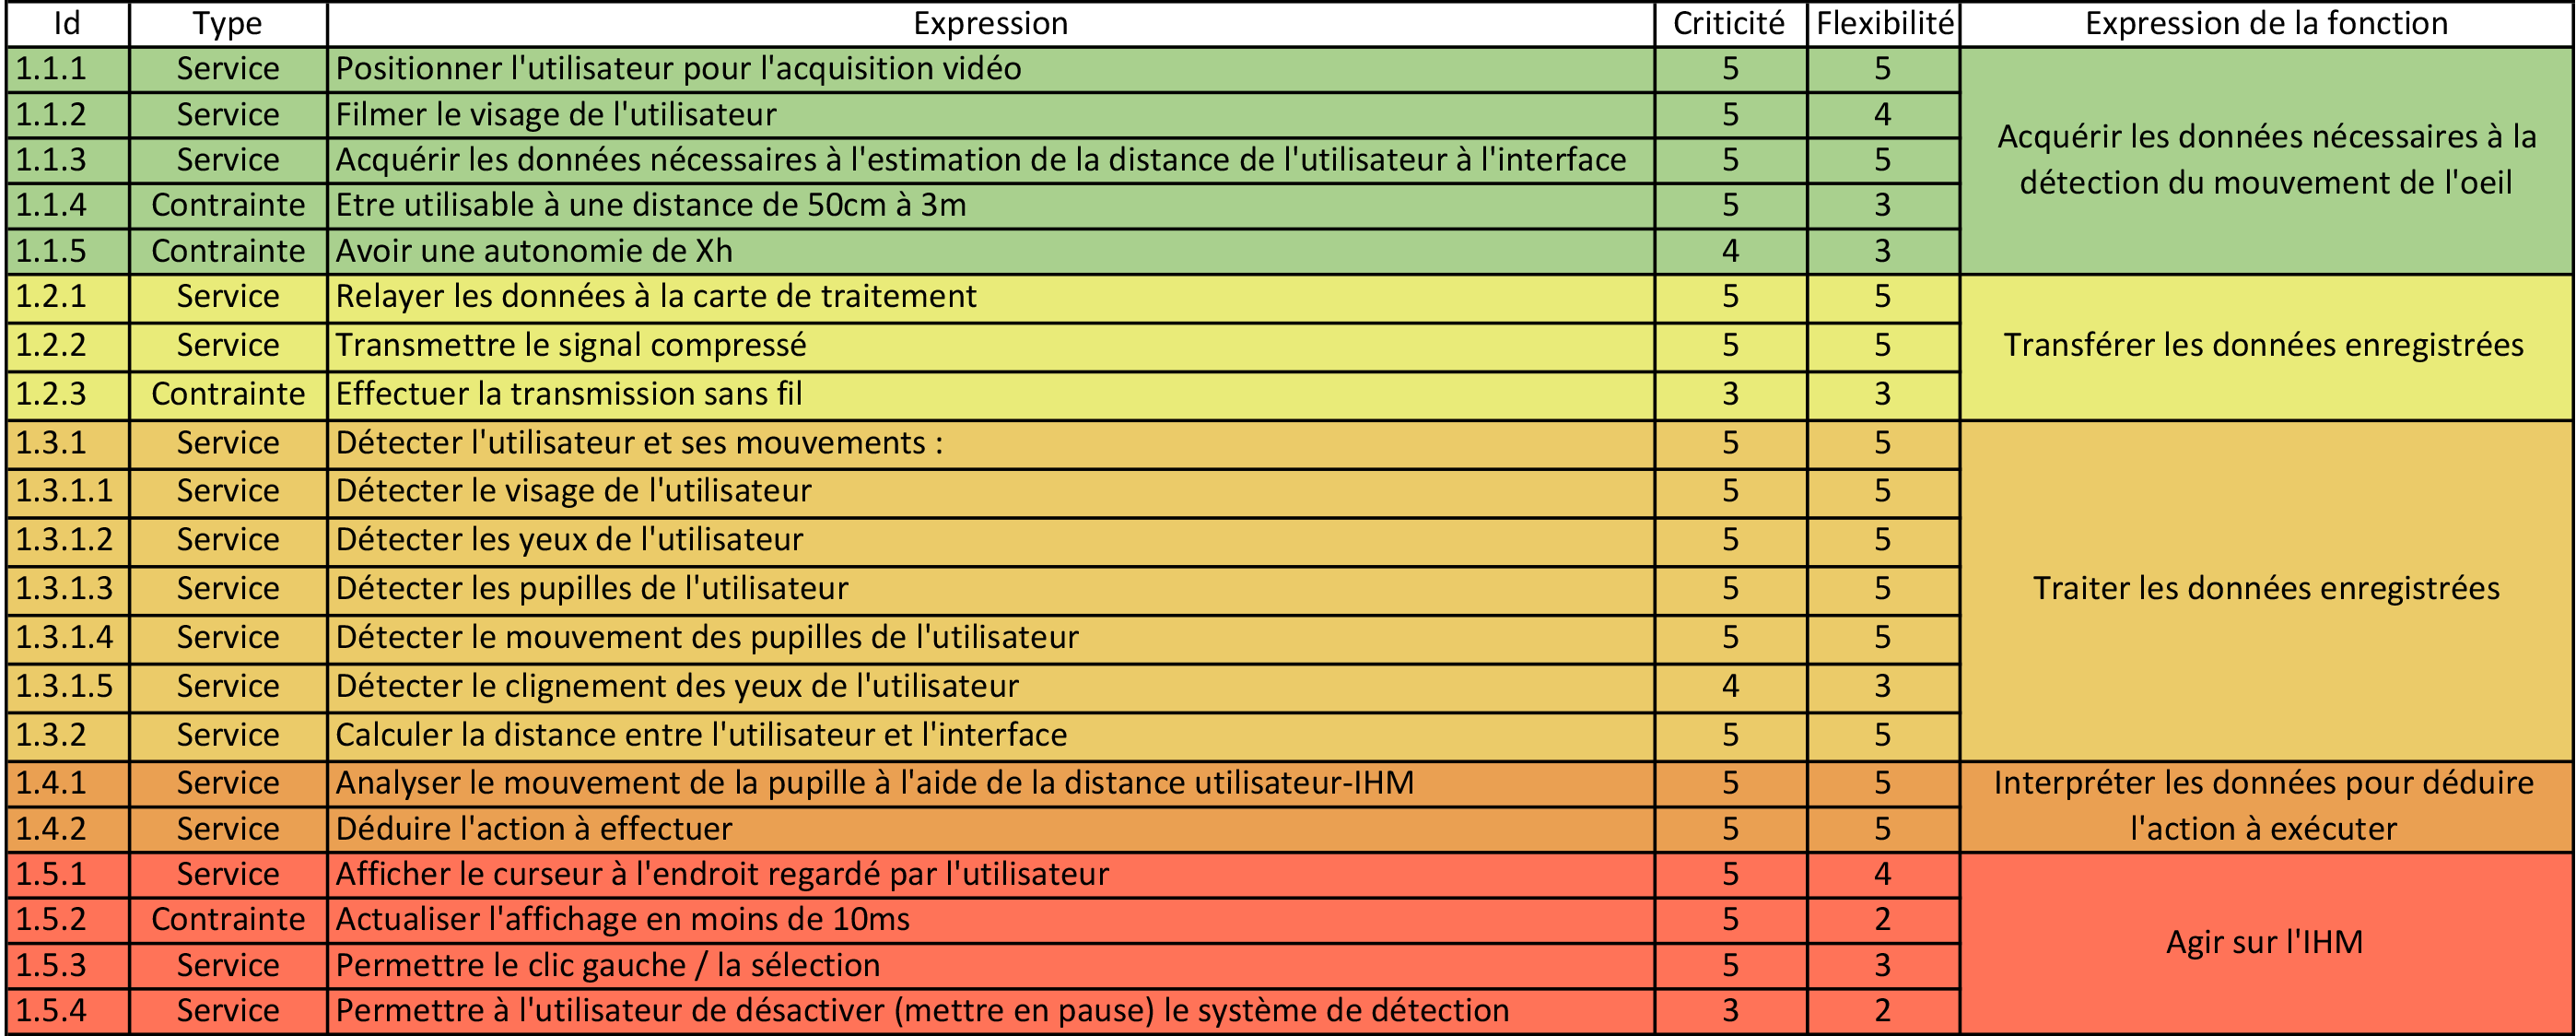
\includegraphics[width=\textwidth]{CahierdesExigences}
  \caption{Cahier des exigences}
  \label{fig:exigences}
\end{figure}

\section{Fonctions principales du système}

\chapter{Spécification fonctionnelle  3 axes}

\section{Raffinement FAST}

\begin{figure}[H]
  \centering
  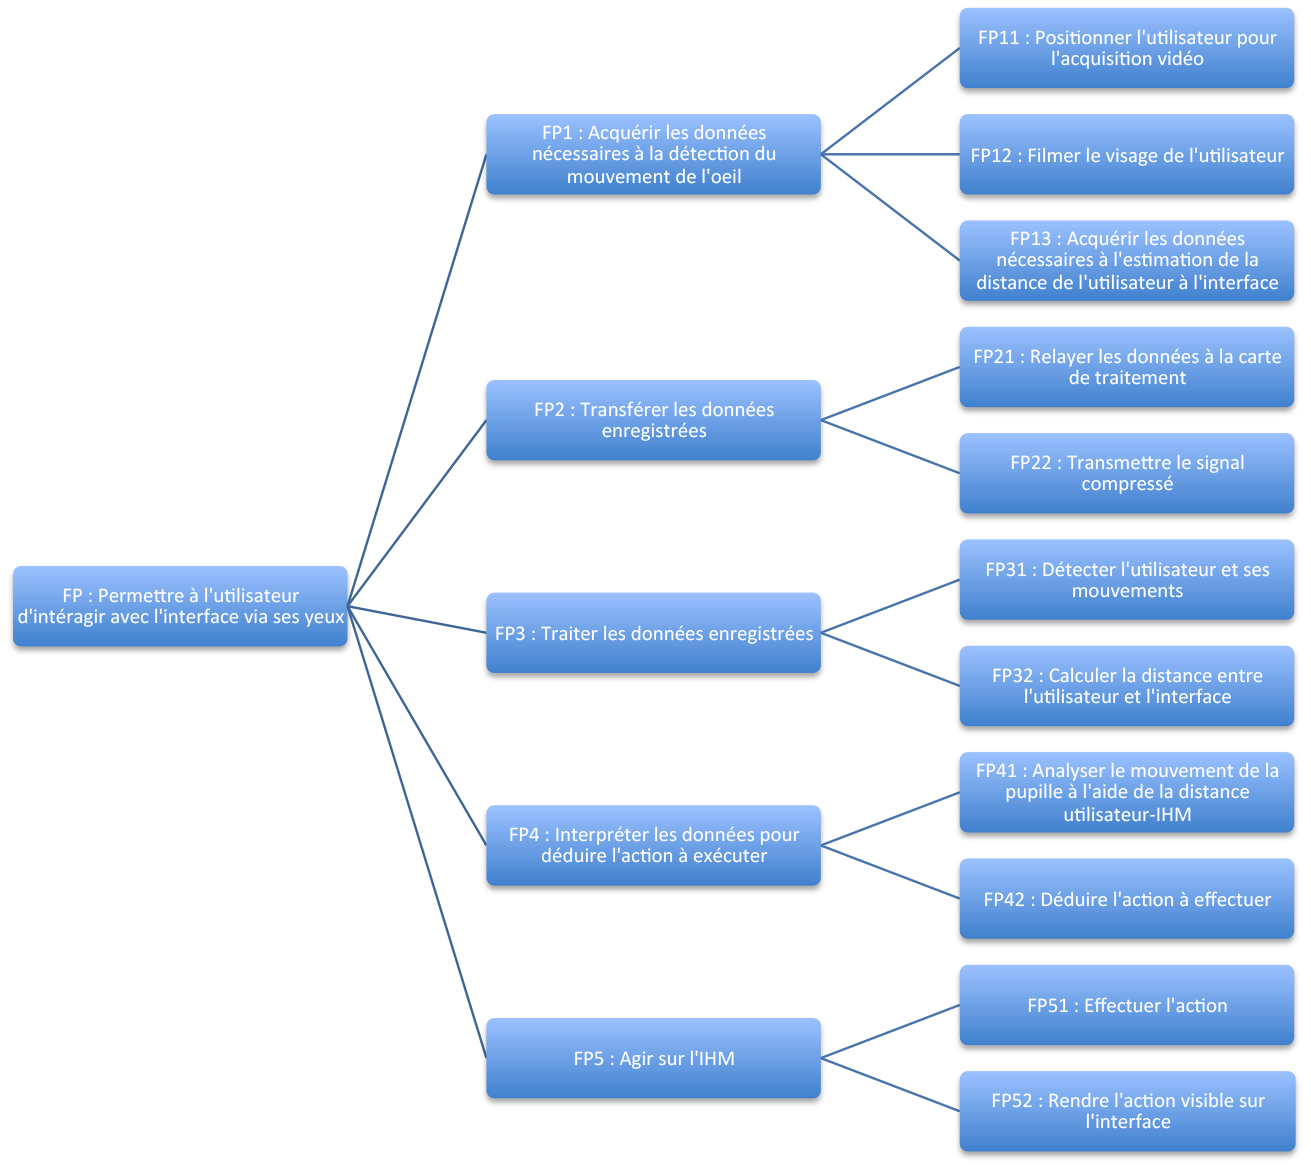
\includegraphics[scale=1.2]{FAST}
  \caption{FAST raffiné}
  \label{fig:FAST}
\end{figure}

\section{Spécification des données}
\section{Spécification des comportements}


\chapter{Architecture fonctionnelle}


